% !TEX encoding = UTF-8 Unicode

\chapter{Introduction}
\label{chap:intro}

%%%%%%%%%%%%%%%%%%%%%%%%%%

\section{Project background}
\label{sec:intro:background}

In 2016, a mobile application named Prisma was launched \cite{wiki:prisma} and became popular rapidly.
The app is attractive to many people because it enables the user to transform your own photo
into artistics effect; e.g.\ make a photo of your cat look like a painting \cite{wiki:prisma}.

    \begin{figure}[!hbt]
    \center
    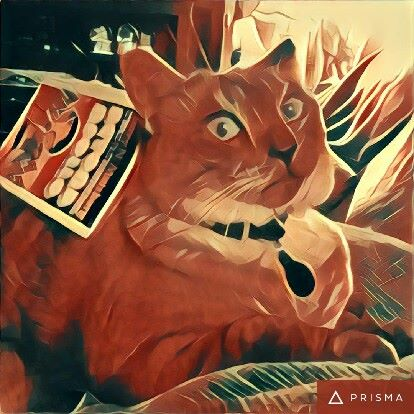
\includegraphics[height=12em]{cat.jpg}
    \caption{An image of a cat rendered via Prisma}
    \label{fig:prisma}
    \end{figure}

The photo-editing app utilizes convolutional neural network techniques to
extract the content and style of two graphs,
and then transfer the artistic style from one to the other,
in order to combine the content of a photo with the style of another.

The artistic style trasfer algorithm was initially proposed in \cite{Gatys:2015ub}
and then published as \cite{Gatys:2016gj}.
This project is intended to implement the algorithm described in \cite{Gatys:2016gj}
(hereinafter referred to as ``the original work'')
and build a Python-Tensorflow based artistic style transfer system
(hereinafter referred to as ``the system'').

One of the biggest differences between this project and other traditional machine learning problems
is that there is not an objective ``accuracy'' measure on the output results.
Combining pictures and paintings is a very subjective process,
and the variation between content and style is adjustable,
as will be stated in Sec.\ \ref{sec:foundation:loss}.

Therefore, chanllenging parts of the project include:
    \begin{enumerate}
        \item Study and parse the large-scale pre-trained deep network data (see Sec.\ \ref{sec:foundation:vgg});
        \item Process images to fit the network;
        \item Define very custom loss functions to ``mix'' the content image and style image.
    \end{enumerate}


%%%%%%%%%%%%%%%%%%%%%%%%%%

\section{Related works}
\label{sec:intro:related}

The topic of artistic transfer has been popular since 2015.
There have been a lot of excellent works and implementations done in the area.
The Prisma app would be a good example.

The authors of \cite{Gatys:2016gj} founded a website named
\texttt{DeepArt.io} themselves \cite{wiki:deepart},
which provides an access for users to upload content and style images.
Another two excellent implementation inspired by the original work
is by JC Johnson on GitHub \cite{Johnson2015}, which is Lua based,
and one by Frank Liu \cite{Liu2017}, which is Python based but
utilizes Sci-Py instead of Tensorflow.

For content representation (content feature extraction) part,
some works have been done in the area of semantic segmentation with convolutional neural network,
among which \cite{Long:2014um} is a good example and referred by the original work.

For style representation (style feature extraction) part,
related works focus on generative networks and texture synthesis \cite{gatys2015texture, Ulyanov:2016tw}.


%%%%%%%%%%%%%%%%%%%%%%%%%%

\section{Development environment and technical specifications}
\label{sec:intro:spec}

The Python-Tensorflow based artistic style transfer system
is built with Python3.6 and Tensorflow1.3.0.
This information along with other Python libraries required to run the code
are all recorded in \texttt{requirements.txt}.
See Appendix \ref{app:readme} for details.

All the examples are generated with a 2012 Macbook Pro laptop.
Table \ref{table:spec} shows some specifications of the laptop,
mainly hardware specs like computing power.

    \begin{table}[!htb]
    \center
    \begin{tabular}{l|l}
    \hline
    \multicolumn{1}{c|}{hardware parameter} & \multicolumn{1}{c}{technical specifications} \\ \hline
    processer (CPU) & 2.9GHz, dual-core Intel Core i7 \\
    memory & 8 GB 1600 MHz DDR3 \\
    graphics (GPU, un-used) & Intel HD Graphics 4000 1024 MB \\
    \hline
    \end{tabular}
    \caption{Technical specification}
    \label{table:spec}
    \end{table}
